%%%%%%%%%%%%%%%%%%%%%%%%%%%%%%%%%%%%%%%%%%%%%%
\logvartrue
\chapter{Bacteria in agro-environments}
%%%%%%%%%%%%%%%%%%%%%%%%%%%%%%%%%%%%%%%%%%%%%%
Soils are dynamic environments and microbes that thrives in these habitats have learned to adapt themselves to changing soil conditions. Currently, most studies of soil bacterial communities focus on the spatial variation in the diversity and composition of soil microbial communities. A relatively large number of these projects have documented that even small changes in land use are able to alter soil bacterial communities and the biological processes they carry out. These changes may even influence the soil productivity in agro-environments leading to a drastic reduction of the annual crop. In order to inspect these microscopical variations due to microscopical factors we should analyse bacterial community in different agronomic environments focusing our attention on the both temporal and spatial scale.\\
These topics has been discussed in the following published paper:
\vspace{-2mm}
\begin{itemize}[nosep]
\item Bevivino, A., Paganin, P., \textbf{Bacci, G.}, Florio, A., Pellicer, M. S., Papaleo, M. C., ... \& Dalmastri, C. (2014). Soil Bacterial Community Response to Differences in Agricultural Management along with Seasonal Changes in a Mediterranean Region. \textit{PloS one}, 9(8), e105515.
\end{itemize}

\section[Soil Bacterial Community Response to Differences in Agricultural Management along with Seasonal Changes in a Mediterranean Region]{Soil Bacterial Community Response to Differences in Agricultural Management along with Seasonal Changes in a Mediterranean Region%
\sectionmark{Soil bacterial response in a Mediterranean agro-environment}}
\sectionmark{Soil bacterial response in a Mediterranean agro-environment}
Soil microorganisms play a crucial role in the maintenance of the major biogeochemical cycles. Indeed, they are able to deeply affect the ecosystem functioning being involved in several biological process ( such as: organic matter dynamics, nutrient cycling and decomposition). To gain insight into the impact of land use on the underlying soil bacterial communities, we aimed at determining the effects of agricultural management, along with seasonal variations, on soil bacterial community in a Mediterranean ecosystem where different land-use and plant cover types led to the creation of a soil and vegetation gradient.\\

\newpage
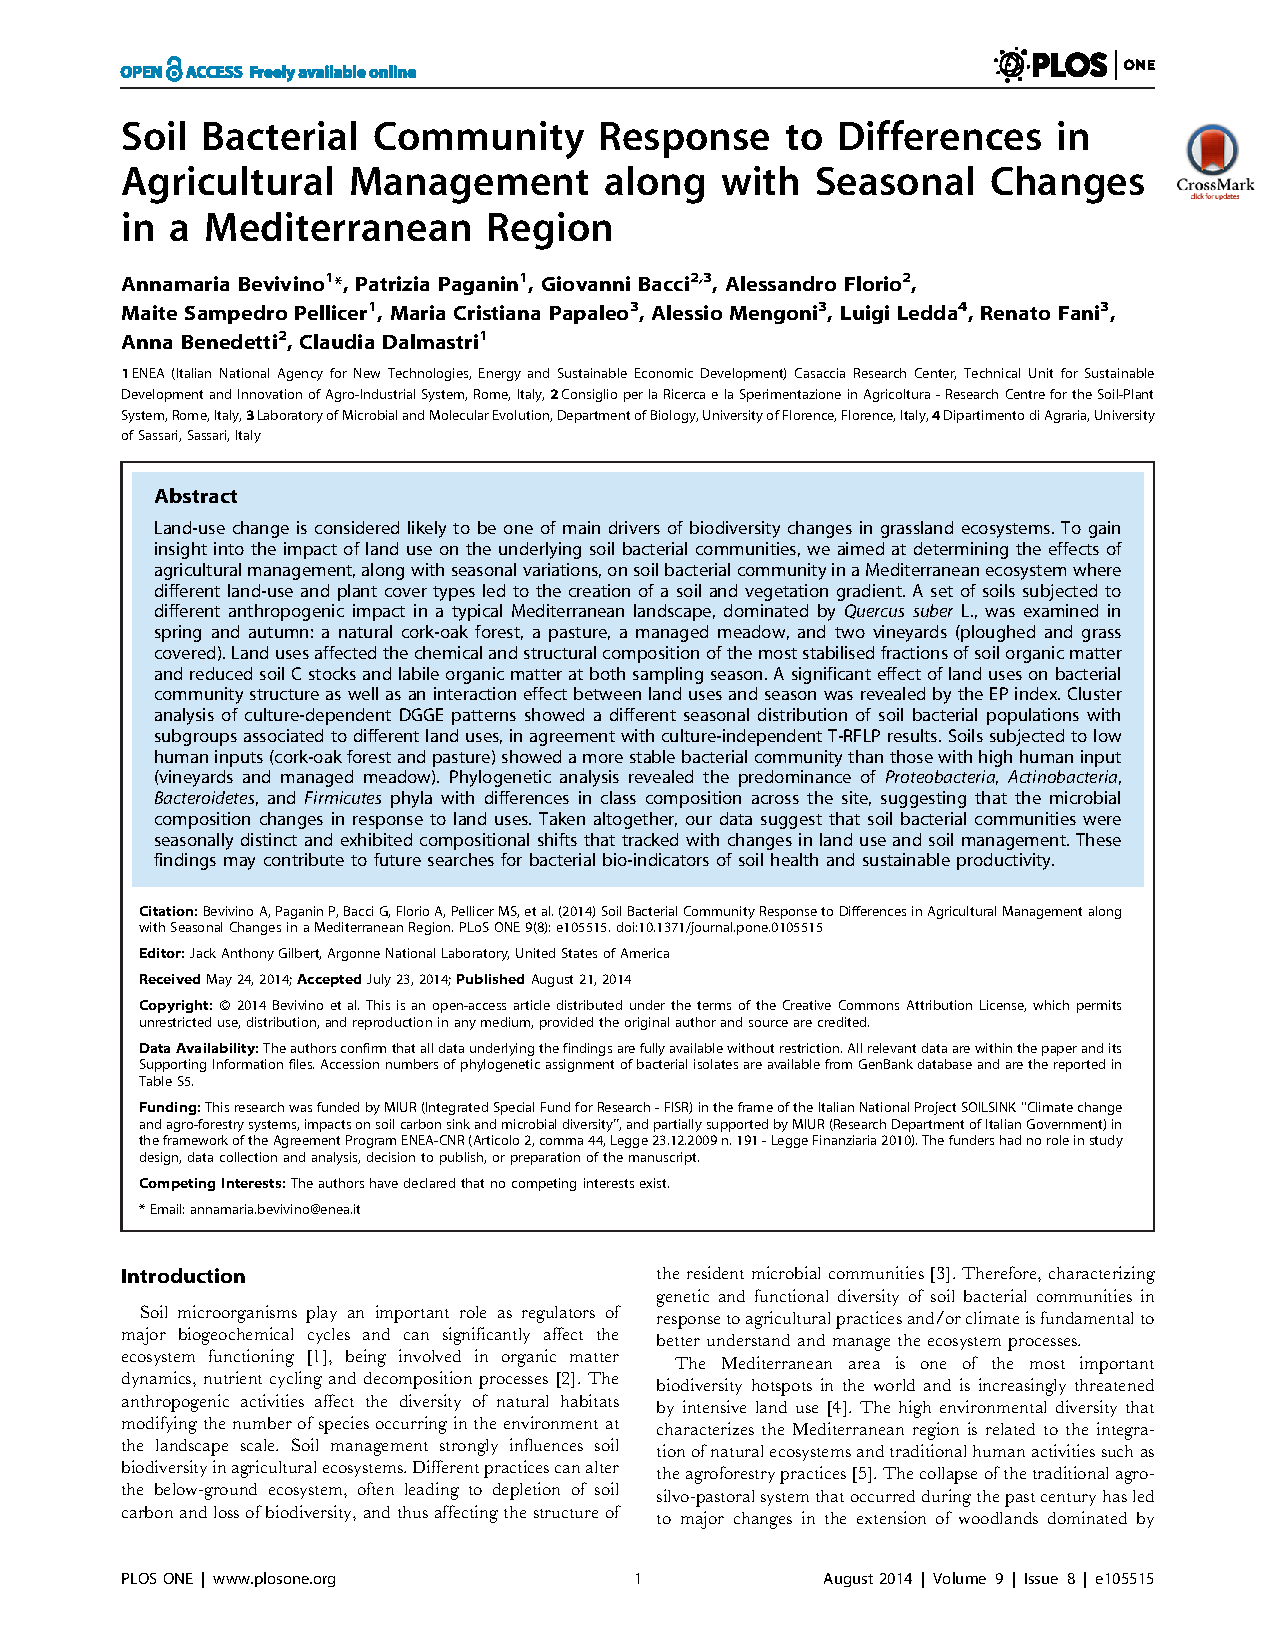
\includepdf[pages=-,offset=10mm 0, scale=0.9]{articles/soil_sink.pdf}
\newpage

%%-----------
%% Backmatter
%%-----------
\backmatter
\chaptermark{Bibliography}
\renewcommand{\sectionmark}[1]{\markright{#1}}
\bibliographystyle{unsrt}                           %Use alpha codes for references
\sectionmark{Bibliography}
\addcontentsline{toc}{chapter}{Bibliography}        %Force addition of Bibliography to TOC    
\bibliography{References}